\documentclass[tikz,border=10pt]{standalone}
\begin{document}
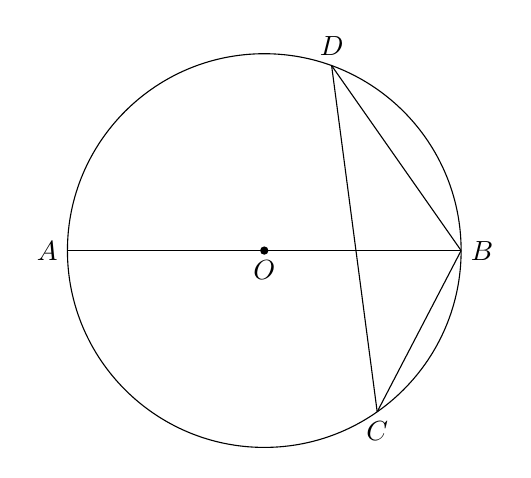
\begin{tikzpicture}
    % Define coordinates
    \coordinate (O) at (0,0);
    \coordinate (A) at (-2.5,0);
    \coordinate (B) at (2.5,0);
    \coordinate (D) at (1.2,2.2); % Approximate position on circle
    \coordinate (C) at (1.5,-2.0); % Approximate position on circle

    % Adjust D and C to be exactly on the circle of radius 2.5
    % Radius r = 2.5.
    % Let's use polar coordinates for precision on the circle
    \coordinate (D) at (70:2.5);
    \coordinate (C) at (-55:2.5);
    \coordinate (A) at (180:2.5);
    \coordinate (B) at (0:2.5);
    \coordinate (O) at (0,0);

    % Draw the circle
    \draw (O) circle (2.5);

    % Draw lines/chords
    \draw (A) -- (B); % Diameter
    \draw (B) -- (D);
    \draw (B) -- (C);
    \draw (C) -- (D);

    % Draw the center point
    \fill (O) circle (1.5pt);

    % Labels
    \node[left] at (A) {$A$};
    \node[right] at (B) {$B$};
    \node[below] at (C) {$C$};
    \node[above] at (D) {$D$};
    \node[below] at (O) {$O$};
\end{tikzpicture}
\end{document}
